\section{Проектные решения конструкции РЭС}

\subsection{Обоснование актуальности разработки \\
  электронного модуля}

В ходе совещания с работниками отдела,
мною был предложен вариант,
когда, основываясь на требованиях сотрудников данного
отдела, я, создавая конструкторскую документацию,
на производства РЭС, ошибки в изготовлении которого не будут
слишком сильно экономически на благополучие фирмы,
но при этом факт успешного изготовления
единичного экземпляра или их пары,
существенно упростил бы работу одного из отделов.

Писать код для ИВК или модернизировать коммуникаторы,
а уж тем более счётчики мне бы не доверили по причине
малого опыта. Поэтому, ко мне пошли на встречу, когда
я предложил выполнить что-то более простое,
но тем не менее полезное отделу сервиса,
в котором я был занят прохождением практики.


Разработка данного радиоэлектронного средства обосновывалась
насущной необходимостью работников предприятия,
которым требовалось устройство упрощающее взаимодействие
между счетчиком и персональным компьютером.

Однако, я тоже сыграл свою роль в таком решение о выборе технического задания.
Дело в том, что компания ООО «РТЕ Сервис» занимается производством
критического оборудования, для которого высока цена ошибки.
Основываясь на этом соображении,
я стремился выбрать проект,
который,
при выполнение с ошибками не принёс бы значительного,
но тем не менее, был бы полезен нескольким работникам предприятия.

\subsection{Составление технического задания\\
  на модернизацию электронного модуля}

Из-за того, 
что я проходил практику не в отделе производства,
а под начальством сотрудников отдела сервиса,
техническое задание на РЭС,
было устно сформулировано работниками сервиса
в устной форме, исходя из требований этого отдела.

Согласно озвученному техническому заданию,
была взята готовая схема преобразователя интерфейсов
\textit{RS-232 - RS-485} из
журнала «Радио Лоцман» ~\cite{rlocman-rs-converter}.

\begin{figure}[H]
  \centering
  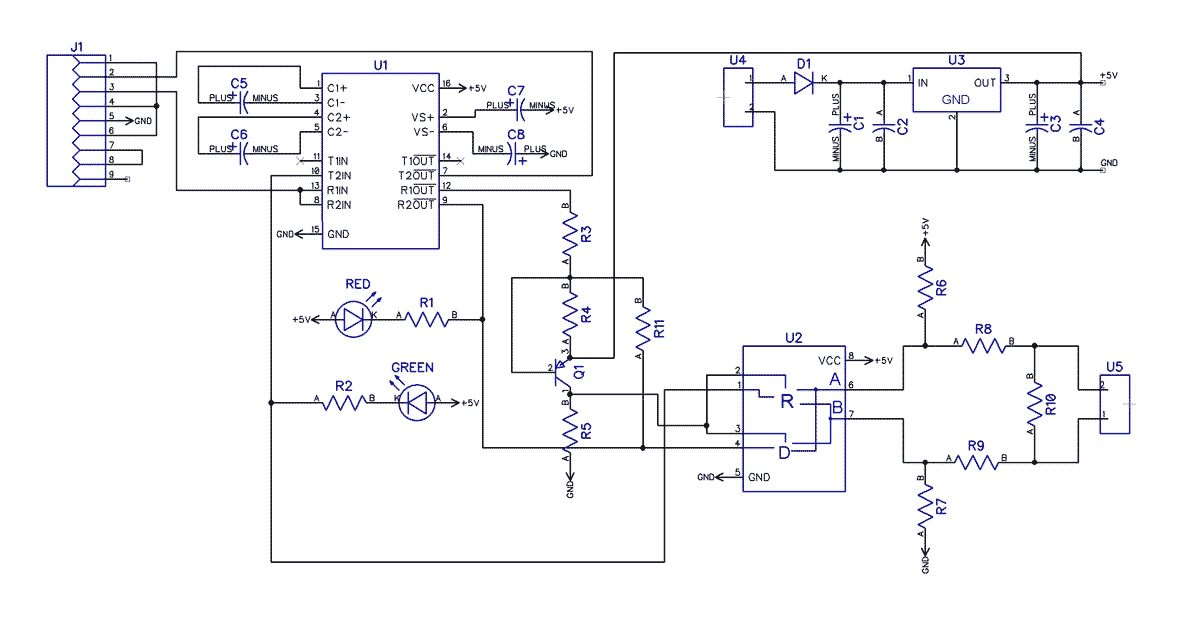
\includegraphics[scale=0.3]{rlocman-schematic.png}
  \caption{Схема представленная на сайте журнала «Радио Лоцман»}
\end{figure}

Модернизация заключалась в том,
что на готовой схеме разъём \textit{DB9}
со стороны включения интерфейса \textit{RS-232}
был заменён на клемму с тремя разъёмами.

Такой выбор был сделан на основании
желания сотрудников раздела
упростить подключение счётчика с интерфейсом \textit{RS-485} к ПК.

Более того: разъём \textit{DB9}
содержит слишком избыточное количество
пинов для подключения по интерфейсу \textit{RS232}.

Конечно же, существуют разные версии стандарта этого интерфейса,
но в минимальной и достаточной комплектации,
необходимы всего три пина:
\begin{itemize}
\item RX
\item TX
\item GND
\end{itemize}

Сам по себе данный стандарт — уточнение
стандарта \textit{UART} и часто, в литературе может быть упомянут как
последовательный порт компьютера.

Недостаток данного интерфейса, в том,
что в отличие от \textit{RS-485}
он не предназначен для передачи данных на дальнее расстояние.
По этой причине на многих старых счетчиках,
изготовленных вне ООО «РТЕ Сервис» был
использован именно этот интерфейс,
как часто вариант размещения,
когда коммуникатор был размещён в одному шкафу с счётчиком,
был недоступен.
В такой ситуации требовалась передача данных на более дальнее расстояние.
И это именно тот случай, когда интерфейс
основанный на принципе работы витой пары,
подходит как никак лучше.


\subsection{Пояснение схемы электрической принципиальной\\
  электронного модуля}

В ходе модернизации схемы её принцип работы не изменился.

Схема, питаемая от блока питания с напряжением пять Вольт
и преобразует сигнал идущий по интерфейсу
стандарта \textit{RS485} в сигнал идущий по интерфейсу
стандарта \textit{RS232}.

\begin{figure}[H]
  \centering
  \includegraphics[scale=0.4]{kicad-rs-converter-sch.pdf}
  \caption{Переработанная, в ходе практики, принципиальная схема.}
\end{figure}


Во время передачи данных микросхема ~\textit{MAX232} преобразует сигнал,
пришедший с клеммы обозначенной,
как «X2» в уровни TTL/CMOS.
Затем микросхема ~\textit{MAX485}
передает этот сигнал в линию \textit{RS-485}, как разность напряжений.
При приеме данных микросхема \textit{MAX485} обнаруживает наличие данных
на линии \textit{RS-485} и передает их микросхеме \textit{MAX232},
после чего сигнал поступает на клеммы.

Красный светодиод показывает передачу,
зеленый – прием данных.

Чтобы обеспечить постоянный уровень напряжения на линии,
когда передача данных не осуществляется,
к ней подключены два резистора.
Один, подключен к напряжению питания, другой к общему проводу ~\cite{rlocman-rs-converter}.

Конвертер управляет режимом приема и передачи автоматически.

\subsection{Выбор элементов и комплектующих изделий для электронного модуля входящего в состав РЭС}

\subsection{Конструкторское проектирование электронного модуля}

\subsection{Компьютерные программы используемые для конструкторского проектирования}
% FreeCAD, SolidWorks
% FlatCAM

\newpage

% Local Variables:
% compile-command: "sh build.sh"
% End:
